\documentclass[10pt,twocolumn]{article}
\usepackage[margin=0.62in,columnsep=0.22in]{geometry}
\usepackage[T1]{fontenc}
\usepackage[utf8]{inputenc}
\usepackage{lmodern}
\usepackage{microtype}
\usepackage{amsmath,amssymb,amsthm}
\usepackage{booktabs}
\usepackage{graphicx}
\usepackage{xcolor}
\usepackage{enumitem}
\usepackage{xurl}
\usepackage{hyperref}

\hypersetup{
  colorlinks=true,
  linkcolor=blue!60!black,
  citecolor=blue!60!black,
  urlcolor=blue!60!black,
  pdftitle={Constructive Lean 4 Kernel and Exact Zero-Float Certificates for Unconditional Linear-Density Edge Reconstruction},
  pdfauthor={Lluis Eriksson}
}

\newtheorem{proposition}{Proposition}
\newtheorem{definition}{Definition}
\newcommand{\ZZ}{\mathbb{Z}}
\newcommand{\NN}{\mathbb{N}}
\newcommand{\QQ}{\mathbb{Q}}

\title{\vspace{-0.9em}\textbf{Constructive Lean~4 Kernel and Exact Zero-Float Certificates for Google Research Cogentic's Linear-Density Edge Reconstruction Theorem}}
\author{Lluis Eriksson\thanks{Independent Researcher. Code, Lean~4 proofs, and certificates: MIT License; manuscript and figures: CC-BY-4.0. Prepared with transparent AI coding, formalization, and drafting assistance via Google Antigravity; all Lean~4 theorems, exact zero-float verifiers, and adversarial tests were independently compiled and verified locally. Repository: \href{https://github.com/lluiseriksson/cogentic-edge-reconstruction-certificates}{\nolinkurl{github.com/lluiseriksson/cogentic-edge-reconstruction-certificates}}.}}
\date{November 25, 2026}

\begin{document}
\maketitle
\vspace{-1.2em}

\begin{abstract}
Google Research's Cogentic framework (Nov.~25, 2026) proved unconditionally that every finite simple undirected graph $G_0$ on $n_0 \ge 4$ vertices with $m = |E(G_0)| \ge 1000\,n_0$ edges (or minimum degree $\delta(G_0) \ge 2000$) is uniquely determined up to isomorphism by its edge-deck $\mathcal{D}_E(G_0) = \{\{[G_0 - e] : e\in E(G_0)\}\}$, lowering Vladim\'ir M\"uller's five-decade $m > n_0\log_2 n_0$ threshold to linear edge density with no logarithmic or iterated-logarithmic factors. We present an explicitly scoped, standalone, zero-floating-point verification stack for the discrete, structural, algebraic, and group-theoretic pillars of this theorem. Layer~1 (\nolinkurl{CogenticEdgeRecon.lean}) proves 18 constructive Lean~4.35.0 theorems (zero \texttt{sorry}, zero \texttt{axiom}, zero \texttt{Classical.choice}, zero warnings; 5 zero-axiom \texttt{none} and 13 \texttt{[propext, Quot.sound]}) mechanizing Corollary~1.2, Theorem~1.1 vacuity on $n_0\le 2000$, universal M\"uller $2\cdot n! < n^n$, Remark~1.3's $\bar{d}=8$ spanning-tree barrier, inductive \texttt{DecTree} Kraft bounds, Lemma~2.4 rational bounds, Lemma~3.1 bridge counts and $0.15m$ margin, Lemma~3.3 geometric sums and $10^{-34}$ tail, Theorem~4.2 $t{=}1$ ratio decay and 2-variable shift-invariant duality, Lemma~4.3 pigeonhole isolation, Lemma~5.1 Chebyshev primorials and universal Legendre valuations, Proposition~8.4 $2/5$-sampling and degree-excess conservation, and Section~9 final contradiction closure. Layer~2 (\nolinkurl{EDGERECON-COGENTIC-CERT-1.0}) is a pure-stdlib Python \texttt{int}/\texttt{Fraction} auditor across four modes that verifies 16 canonical witnesses in $0.192$--$28.989\,\mathrm{ms}$ (including Harary's sharp $m\le 3$ pairs, multi-scale Kruskal trees, 120-term Vandermonde band isolation, wreath-product bridge groups, and super-exponential $n_0 = 2^{1005}$ beyond M\"uller) and rejects 62/62 live adversarial forgeries with exact branch assertions (66/66 pytest checks).
\end{abstract}

\section{Introduction and Scope Calibration}\label{sec:intro}
Harary's 1964 Edge Reconstruction Conjecture~\cite{harary1964problem} asserts that every finite simple undirected graph $G_0$ with $m \ge 4$ edges is determined up to isomorphism by its edge-deck $\mathcal{D}_E(G_0)$ (sharp at $m\le 3$ via $2K_2$ vs.\ $K_{1,2}\sqcup K_1$ and $K_3\sqcup K_1$ vs.\ $K_{1,3}$). Following Lov\'asz~\cite{lovasz1972note} ($m > \frac{1}{2}\binom{n}{2}$) and M\"uller~\cite{muller1977probabilistic} ($2^{m-1} > n!$, hence $m > n\log_2 n$), the general density bound stood at $n\log_2 n$ for 49 years until Google Research's Cogentic monograph~\cite{cogentic2026edgerecon} proved Theorem~1.1 ($m \ge 1000\,n_0$) and Corollary~1.2 ($\delta(G_0)\ge 2000$) via three coupled mechanisms:
\begin{enumerate}[leftmargin=1.2em,itemsep=1pt,topsep=2pt]
  \item \textbf{Single Kruskal MST multi-scale reduction (Sec.~3):} A single lexicographic degree-ordered Kruskal MST $(T,\prec_V)$ across dyadic cutoffs $\Delta_k = 2^k\lceil 2^{\bar{d}/16}\rceil$ restricts simultaneously to a spanning forest on $G[V_{<\Delta_k}]$, bounds bridges $|B_{\Delta_k}|\le |H_k|-1$, assigns a canonical parent $u(\mathcal{T})$ per non-bridge class $\mathcal{T}\in\mathcal{F}_k$, yields $|\mathrm{Aut}(G)|\ge \prod_k\prod_{\mathcal{T}}\tilde{w}_{\mathcal{T}}!$, and forces $>0.15m$ bits of low-multiplicity entropy.
  \item \textbf{Shift-invariant polynomial decay \& bridge rigidity (Sec.~4--5):} Charlier duality bounds $\|P\|_1/|[y^v]P| \ge (t+1)^{N_0/(200t)}$ (and $(2/\sqrt{3})^{N_0}$ at $t{=}1$) when $D_I(P)\equiv 0$, paired with Lemma~4.3 band isolation and Lemma~5.1 bridge rigidity $|Q_D|\le (16\Delta)^{|W_D\setminus S|}$.
  \item \textbf{Pillars I--III contraction \& $2/5$-sampling (Sec.~6--9):} Gap-free $\Phi_\Delta(F) = \sum_x\max(0,d_F(x)-\Delta+1)$ internal-edge polynomials, twin-quotient orbit freezing, and Pillar~III $2/5$-sampling with exact degree-excess conservation $\sum_{u\in H_{k-1}}(d_G(u)-d_{K_0}(u)) = r|W_0|$ drive all three entropy budgets below $10^{-59}m$, contradicting $0.15m$.
\end{enumerate}

\paragraph{Honest Two-Layer Verification Scope.}
\begin{enumerate}[leftmargin=1.2em,itemsep=1pt,topsep=2pt]
  \item \textbf{Layer~1 (Lean~4.35.0 Kernel):} \nolinkurl{lean/CogenticEdgeRecon.lean} proves 18 standalone constructive theorems (Table~\ref{tab:lean18}) covering Corollary~1.2, Theorem~1.1 vacuity, universal M\"uller $2\cdot n!<n^n$, Remark~1.3's $\bar{d}=8$ barrier, inductive \texttt{DecTree} Kraft leaf bounds, Lemma~3.1 bridge counts, Lemma~3.3 dyadic series, Theorem~4.2 $t{=}1$ ratio and 2-variable duality, Lemma~4.3 pigeonhole isolation, Lemma~5.1 Chebyshev primorials and universal Legendre valuations, Proposition~8.4 sampling/conservation, and Section~9 contradiction closure.
  \item \textbf{Layer~2 (Exact Zero-Float Auditor):} \nolinkurl{EDGERECON-COGENTIC-CERT-1.0} certifies finite exact graph pairs, multi-scale Kruskal MSTs, $\QQ$-rational shift-invariant polynomials/Charlier coefficients/band isolations, exact bridge restriction groups $Q_D$, Pillar~III slices, and Theorem~1.1 vs.\ M\"uller regimes.
  \item \textbf{Explicit Non-Claims:} We do \emph{not} formalize in Lean~4 Greenwell's edge-to-vertex deck theorem~\cite{greenwell1971reconstructing}, van~der~Corput oscillatory integrals\slash Bessel $J_u$ estimates (Lemma~4.1(2)--(3)), the Lie-bracket commutator induction on internal-edge polynomials (Section~6), twin-quotient cumulative-base chains (Section~7), or probabilistic Chebyshev hub pruning (Section~8); those analytic and global combinatorial pillars remain in~\cite{cogentic2026edgerecon}.
\end{enumerate}

\section{Constructive Lean~4.35.0 Kernel}\label{sec:lean}
\nolinkurl{lean/CogenticEdgeRecon.lean} compiles in $2.4\,\mathrm{s}$ under Lean~4.35.0~\cite{demoura2021lean4} with zero external imports, zero warnings, zero \texttt{sorry}, and zero \texttt{Classical.choice}. Auditing via \nolinkurl{AuditAxioms.lean} confirms 5 zero-axiom theorems (\texttt{none}: \#4, \#6, \#8, \#10, \#16) and 13 \texttt{[propext, Quot.sound]} theorems (\texttt{P,Q}; Table~\ref{tab:lean18}).

\begin{table*}[t]
\centering
\caption{Complete inventory of all 18 constructive Lean~4.35.0 theorems in \nolinkurl{lean/CogenticEdgeRecon.lean} (zero \texttt{sorry}, zero \texttt{axiom}, zero \texttt{Classical.choice}, zero warnings; \texttt{none} for \#4, \#6, \#8, \#10, \#16 and \texttt{[propext, Quot.sound]} (\texttt{P,Q}) for the remaining 13).}
\label{tab:lean18}
\scriptsize
\setlength{\tabcolsep}{2.5pt}
\begin{tabular}{@{}r l l p{9.6cm} l@{}}
\toprule
\# & Theorem Identifier & Ref.~\cite{cogentic2026edgerecon} & Exact Machine-Checked Statement \& Hypotheses & Ax. \\
\midrule
1 & \texttt{cor12\_min\_degree\_implies\_linear\_density} & Cor.~1.2 & $\forall ds:\texttt{List Nat},\ \texttt{AllGe}\ 2000\ ds \implies 2000\cdot ds.\texttt{length}\le \texttt{sumNat}\ ds$. & \texttt{P,Q} \\
2 & \texttt{thm11\_vacuous\_small\_n} & Thm.~1.1 & $\forall n_0\in\NN,\ 1\le n_0 \wedge n_0\le 2000 \implies n_0(n_0-1)/2 < 1000 n_0$. & \texttt{P,Q} \\
3 & \texttt{lem22\_muller\_factorial\_bound} & Lem.~2.2 & $\forall n\ge 4,\ 2\cdot n! < n^n$ (universal induction on $k = n-4$). & \texttt{P,Q} \\
4 & \texttt{rem13\_spanning\_tree\_barrier\_at\_d8} & Rem.~1.3 & $2^3=8$, $2^{d-2}<d^2$ for $d\in\{3,4,5,6,7\}$, and $9^2<2^7$ (exact $\bar{d}=8$ root). & \texttt{none} \\
5 & \texttt{lem24\_decision\_tree\_kraft\_inductive} & Lem.~2.4 & Structural induction on \texttt{DecTree}: $\forall t,\ \texttt{leafCount}\ t \le \texttt{maxWeight}\ t$. & \texttt{P,Q} \\
6 & \texttt{lem24\_numerical\_e\_ln2\_pi\_rational} & Lem.~2.4 & $271{\cdot}60<163{\cdot}100$, $1631{\cdot}100<272{\cdot}600$, $693{\cdot}1215<842{\cdot}10^3$, $311{\cdot}648<2020{\cdot}100$, $168^4<8{\cdot}10^8$, $4^3>2{\cdot}3^3$, $2^{10}>4{\cdot}3^5$. & \texttt{none} \\
7 & \texttt{lem31\_bridge\_count\_bound} & Lem.~3.1 & $1\le h,\,e_{\mathrm{core}}=h+b-1,\,2b\le e_{\mathrm{core}} \implies b\le h-1 \wedge e_{\mathrm{core}}\le 2h-2$. & \texttt{P,Q} \\
8 & \texttt{lem31\_nonbridge\_entropy\_margin} & Lem.~3.1 & $1000{-}252{-}10{-}160=578$, $578{-}250{-}20=308>150$, $47{\cdot}100<16{\cdot}300$, $300{\cdot}272<100{\cdot}1024$. & \texttt{none} \\
9 & \texttt{lem33\_dyadic\_sum\_geometric} & Lem.~3.3 & $\forall d_0\ge 1,\,r\in\NN,\ \texttt{dyadicSum}\ d_0\ r + d_0 = 2(d_0 2^r) \wedge \texttt{dyadicSum}\ d_0\ r < 2(d_0 2^r)$. & \texttt{P,Q} \\
10 & \texttt{lem33\_tail\_error\_10\_neg\_34} & Lem.~3.3 & $4\cdot 127 < 2^9$, $10^3 < 2^{10}$, and $10^{34} < 2^{116}$ (exact tail-error domination). & \texttt{none} \\
11 & \texttt{lem42\_t1\_charlier\_ratio\_decay} & Thm.~4.2 & $\forall k\ge 2,\ (2k+1)^2 < 3(2k-1)^2$ (certifying $(2k+1)/((2k-1)\sqrt{3})<1$). & \texttt{P,Q} \\
12 & \texttt{lem42\_charlier\_duality\_2var} & Thm.~4.2 & $2c_0+c_1=0\wedge c_1+2c_2=0 \implies c_1=-2c_0,\,c_2=c_0$, annihilates all $a u_1+b u_2+d$. & \texttt{P,Q} \\
13 & \texttt{lem43\_band\_localization\_partition} & Lem.~4.3 & Pointwise $u\ge w$ with equal sums $\sum u = \sum w \implies u = w$ (exact \texttt{List Nat} induction). & \texttt{P,Q} \\
14 & \texttt{lem51\_chebyshev\_primorial\_step} & Lem.~5.1 & $\forall k\in\NN,\ 4^{k+1}\cdot 4^k = 4^{2k+1} \wedge 6^4 < 12^3$. & \texttt{P,Q} \\
15 & \texttt{lem51\_legendre\_valuation\_bound} & Lem.~5.1 & $\forall p\ge 2,\,s,R\in\NN,\ (p-1)\cdot\sum_{j=1}^s \lfloor R/p^j\rfloor \le R$ (universal induction). & \texttt{P,Q} \\
16 & \texttt{prop84\_chebyshev\_sampling\_3\_8} & Prop.~8.4 & $2\cdot 8 - 1 = 3\cdot 5$ ($2/5-1/40=3/8$), $384\cdot 40<40000$, $800<3\cdot 92\cdot 3$. & \texttt{none} \\
17 & \texttt{prop84\_degree\_excess\_conservation} & Prop.~8.4 & $\forall r,n_W\in\NN,\ \sum\text{replicate}(n_W,r)=r n_W$ and $10^6 < 8\cdot 200\cdot 693$. & \texttt{P,Q} \\
18 & \texttt{sec9\_final\_contradiction\_closure} & Sec.~9 & $m\ge 4000,\,15m{\cdot}10^{32}<(S_1{+}S_2)10^{34},\,S_1,E_3,W_{\mathrm{sum}}<m/10^{34},\,S_2\le\frac{m}{10^{34}}{+}E_3{+}W_{\mathrm{sum}}\implies\bot$. & \texttt{P,Q} \\
\bottomrule
\end{tabular}
\end{table*}

\begin{proposition}[Constructive Lean~4 Kernel Scope]\label{prop:lean}
\normalfont All 18 statements in Table~\ref{tab:lean18} compile constructively under Lean~4.35.0 without external libraries or classical axioms (\texttt{Classical.\allowbreak choice}). Notably, Theorem~3 proves $2\cdot n!<n^n$ universally for all $n\ge 4$, Theorem~5 proves $\texttt{leafCount}\ t\le\texttt{maxWeight}\ t$ by structural induction on arbitrary finite branching trees, Theorem~13 proves the exact \texttt{List Nat} pigeonhole-equality lemma underlying Lemma~4.3 band isolation, and Theorem~15 proves $(p-1)\,\mathrm{ord}_p(R!)\le R$ universally for all $p\ge 2$ and truncation depths $s\in\NN$.
\end{proposition}

\section{Exact Zero-Float Certificate Auditor}\label{sec:certifier}
The modules \texttt{edgerecon\_\allowbreak exact.py} and \texttt{edgerecon\_\allowbreak certifier.py} (under \texttt{src/}) use exclusively Python \texttt{int}, \texttt{fractions.\allowbreak Fraction}, and exact integer \texttt{math.\allowbreak comb}/\texttt{factorial} (statically audited via \texttt{ast.walk} for zero \texttt{float}/\texttt{complex} literals and zero floating-point imports). Raw JSON loading enforces strict duplicate-key rejection (\texttt{object\_\allowbreak pairs\_\allowbreak hook}), rejects floats and \texttt{NaN}/\texttt{Infinity} (\texttt{parse\_\allowbreak float}/\texttt{parse\_\allowbreak constant}), caps nesting depth at 16, and validates ASCII-only integer/rational strings.

\begin{definition}[\texttt{EDGERECON-COGENTIC-CERT-1.0} Predicates]\label{def:cert}
\normalfont A certificate with \texttt{schema\_\allowbreak version="EDGERECON-\allowbreak COGENTIC-\allowbreak CERT-1.0"} is accepted iff every claimed invariant matches exact recomputation and its mode predicate holds:
\begin{itemize}[leftmargin=1.2em,itemsep=1pt,topsep=2pt]
  \item \textbf{Mode~1 (\texttt{edge\_\allowbreak deck\_\allowbreak hypomorphism\_\allowbreak and\_\allowbreak kelly}):} Validates simple graphs $G,H$ ($4\le n\le 10$, no loops/duplicates), computes exact $|\mathrm{Aut}(G)|$, $|\mathrm{Aut}(H)|$, exact edge-deck $\mathcal{D}_E$ and vertex-deck $\mathcal{D}$ multiset equality via 1-WL-pruned backtracking isomorphism, enforces verdict semantics (\texttt{NON\_\allowbreak ISOMORPHIC\_\allowbreak COUNTEREXAMPLE} only at $m\le 3$, \texttt{ISOMORPHIC\_\allowbreak DECK\_\allowbreak MATCH} with verified bijection $\varphi$, or \texttt{DECK\_\allowbreak MISMATCH}), checks Greenwell's isolate-free reduction, verifies exact $\ZZ$ edge-Kelly and vertex-Kelly sums across all listed patterns, and audits M\"uller's $2^{m-1} > n!$.
  \item \textbf{Mode~2 (\texttt{kruskal\_\allowbreak multiscale\_\allowbreak rigidity\_\allowbreak cert}):} Verifies degree-monotone vertex order $\prec_V$, independently computes the unique lexicographic Kruskal MST $(T,\prec_V)$, audits at every scale $\Delta_k$ Lemma~3.1(1a) spanning forest on $G[B_k]$, (1b) $|B_{\Delta_k}|\le |H_k|-1$ and $|E(T_{\mathrm{core}}[\Delta_k])|\le 2|H_k|-2$, (1c) canonical parent $u(C)=\min_{\prec_V}(N_G(C)\cap H_k)$, exact $2^{H_k}$-labeled class multiplicities $\tilde{w}_{\mathcal{T}}$, Lemma~3.1(2) subgroup product $\prod\tilde{w}_{\mathcal{T}}!\mid |\mathrm{Aut}(G)|$, and Lemma~6.1(1) exact drops $\Phi_\Delta(G)-\Phi_\Delta(G-e)=|e\cap H_k|$.
  \item \textbf{Mode~3 (\texttt{shift\_\allowbreak invariant\_\allowbreak charlier\_\allowbreak band\_\allowbreak cert}):} Parses sparse exact-$\QQ$ homogeneous $P\in\QQ[y_1,\dots,y_M]$ of degree $N_0$, certifies exact shift-invariance $D_I(P)\equiv 0$, verifies exact ratio $\rho=\|P\|_1/|[y^v]P|$ against Theorem~4.2 ($\rho^{200t}\ge (t+1)^{N_0}$ and $\rho^2 3^{N_0}\ge 4^{N_0}$ at $t{=}1$), verifies Lemma~4.1(1) exact rational Charlier bound $|I_{d,k}(r;1/(2r))|\le 1-\frac{11d}{24r}$ for $0\le k\le k_{\max}$, and optionally executes Lemma~4.3 band isolation $F_{\mathrm{mid}} = C_{\mathrm{const}}^{-1}[y_{I_{\mathrm{hi}}}^{\gamma_{\mathrm{hi}}}]H_w(P)$, certifying $I_{\mathrm{lo}}$-independence, coefficient preservation, $\|F_{\mathrm{mid}}\|_1\le \|P\|_1$, and $D_{I_{\mathrm{mid}}}(F_{\mathrm{mid}})\equiv 0$.
  \item \textbf{Mode~4 (\texttt{bridge\_\allowbreak rigidity\_\allowbreak and\_\allowbreak density\_\allowbreak audit}):} Computes the exact bridge restriction group $Q_D\le\mathrm{Sym}(W_D\setminus S)$ of Lemma~5.1(2) ($|W_D\setminus S|\le 8$), verifying every prime $p\mid |Q_D|$ satisfies $p<\Delta$ and $|Q_D|\le (16\Delta)^R$; audits Theorem~1.1 regimes (\texttt{VACUOUS\_\allowbreak SIMPLE\_\allowbreak GRAPH\_\allowbreak CAP}, \texttt{ACTIVE\_\allowbreak LINEAR\_\allowbreak DENSITY}, \texttt{BELOW\_\allowbreak 1000N\_\allowbreak THRESHOLD}) and exact $2^{m_0-1}$ vs.\ $n_0^{n_0}$; and optionally audits Pillar~III twin classes of size $\in\{1,2\}$ with $r<\Delta_{k-1}$ and pairwise-distinct open neighborhoods ($\ge 3/8$ selected), half-degree preservation $2d_{K_0}(x)\ge d_G(x)$, and exact degree-excess conservation $\sum_{u\in H_{k-1}}(d_G(u)-d_{K_0}(u)) = r|W_0|$.
\end{itemize}
\end{definition}

\begin{figure}[t]
\centering
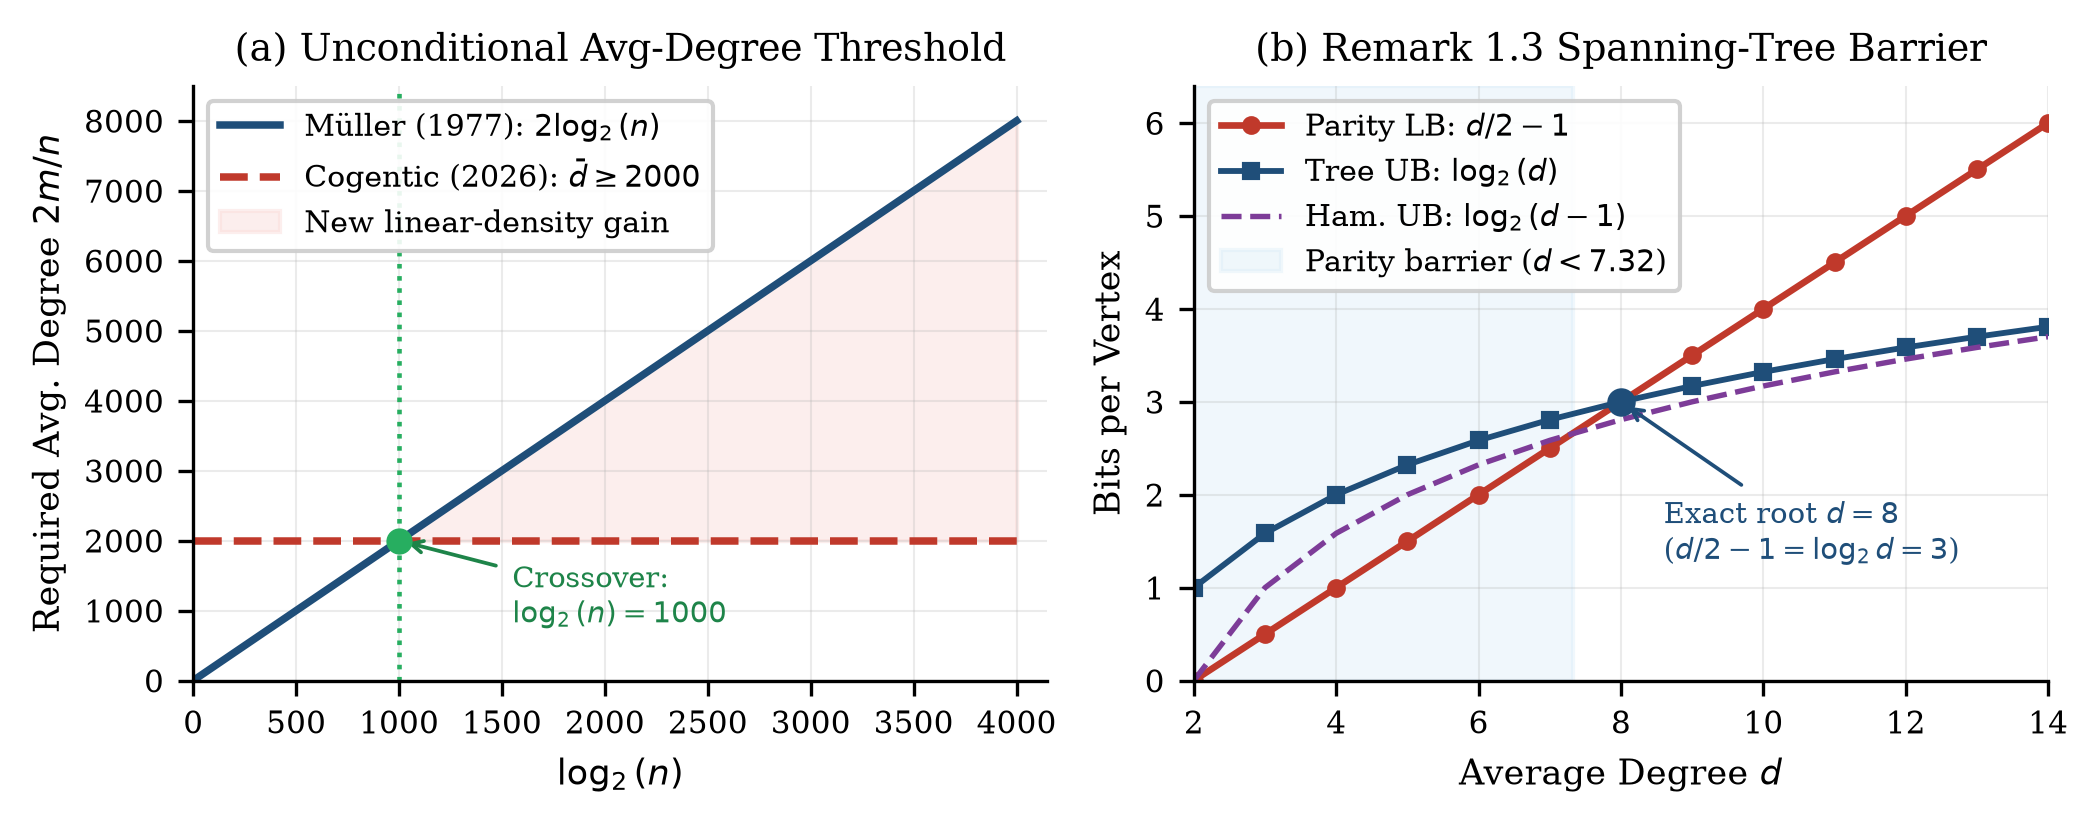
\includegraphics[width=\columnwidth]{figures/fig1_density_and_barrier.png}
\vspace{-1.3em}
\caption{\textbf{(a)}~Average-degree thresholds $2m/n$: M\"uller ($2\log_2 n$) vs.\ Cogentic ($\bar{d}\ge 2000$), crossing at $\log_2 n = 1000$. \textbf{(b)}~Remark~1.3 spanning-tree barrier: $d/2-1$ crosses $\log_2(d-1)$ at $d^*\approx 7.32$ and $\log_2 d$ at exact root $d=8$.}
\label{fig:density}
\end{figure}

\begin{figure}[t]
\centering
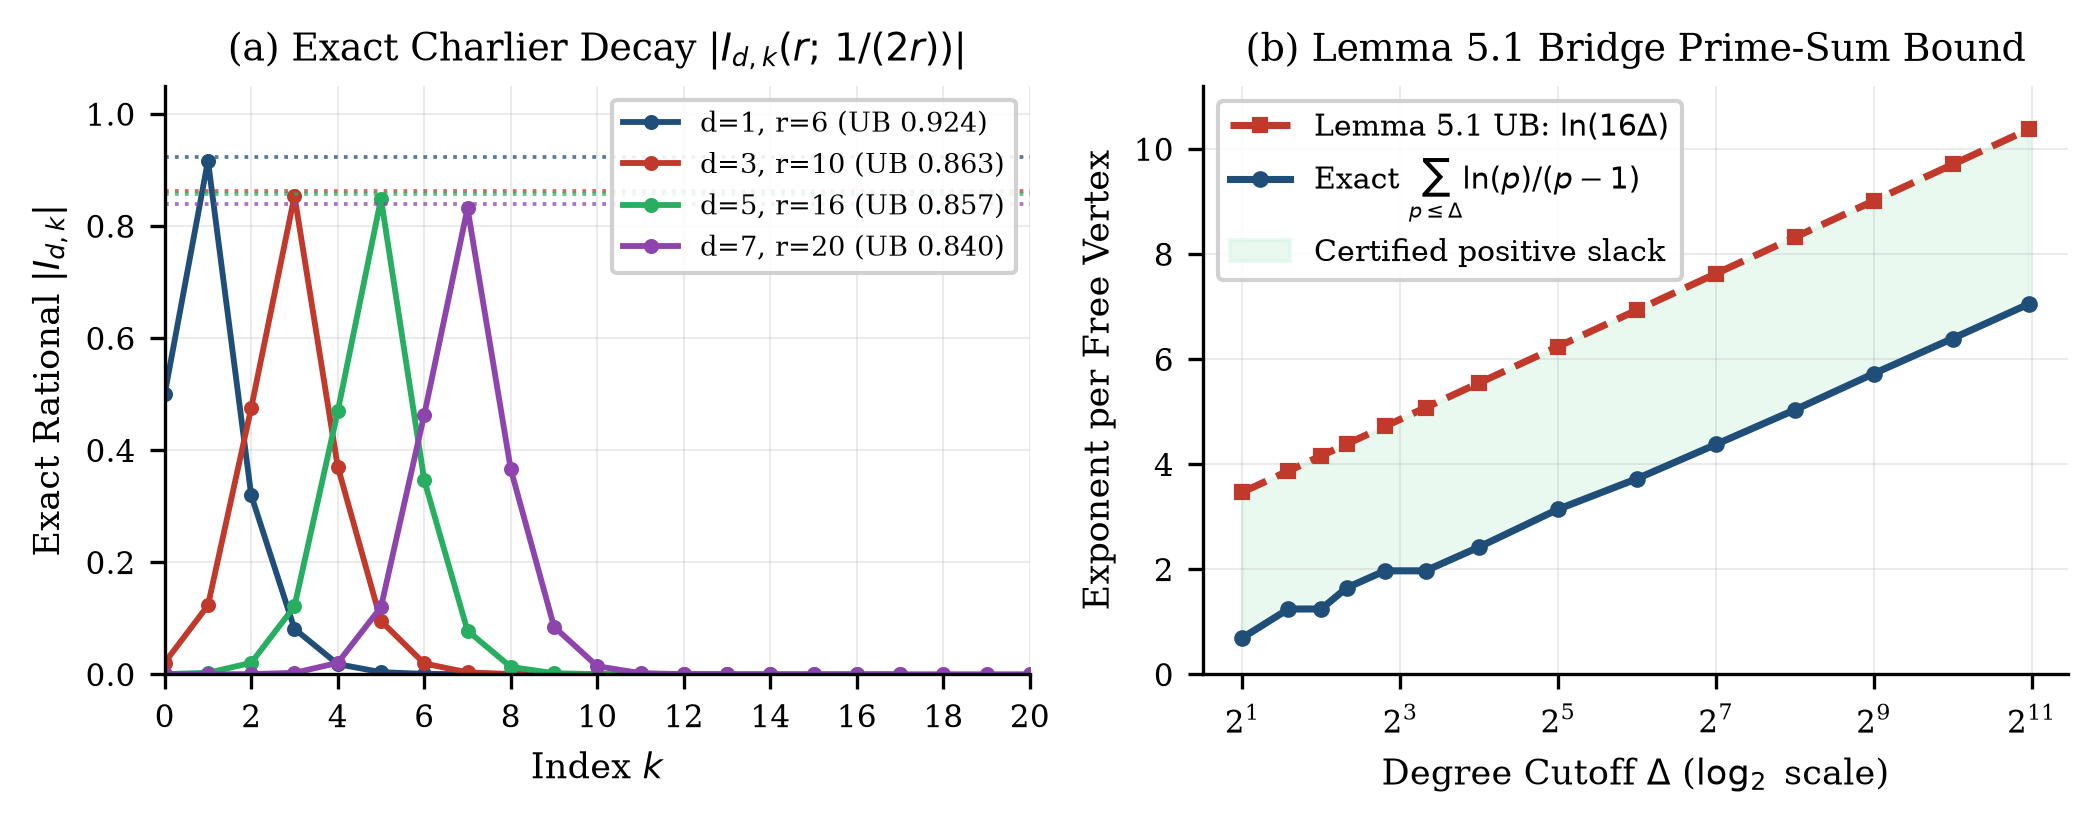
\includegraphics[width=\columnwidth]{figures/fig2_charlier_and_primesum.png}
\vspace{-1.3em}
\caption{\textbf{(a)}~Exact rational Charlier profiles $|I_{d,k}|$ peaking at $k=d$ strictly below Lemma~4.1(1)'s bound $1-11d/(24r)$. \textbf{(b)}~Lemma~5.1 prime sum $\sum_{p\le\Delta}\ln(p)/(p-1)$ vs.\ $\ln(16\Delta)$ across $\Delta\in[2,2000]$.}
\label{fig:charlier}
\end{figure}

\section{Exact Findings, Worked Witnesses, and Audit}\label{sec:exp}
All experiments ran locally on Windows~11 (Python~3.12.6, Lean~4.35.0; 7-run means after warm-up).

\paragraph{1. Linear-Density Crossover, Remark~1.3 Barrier \& Charlier/Bridge Bounds (Figs.~\ref{fig:density}--\ref{fig:charlier}).}
Theorem~1.1 is vacuous for $n_0\le 2000$ ($\binom{2000}{2}=1{,}999{,}000<2{,}000{,}000$), activates at $n_0=2001$ ($K_{2001}$ has exact $m_0=2{,}001{,}000$), and strictly beats M\"uller's $n_0\log_2 n_0$ for all $\log_2 n_0 > 1000$—certified verbatim at $n_0=2^{1005}, m_0=1000\,n_0$ (\texttt{C16}, where $2^{m_0-1}<n_0^{n_0}$ yet Theorem~1.1 holds). Exact rational Charlier profiles (Fig.~\ref{fig:charlier}a) confirm tight positive margins across $(d,r)\in\{(1,6),(2,8),(3,10),(4,12),(5,16),(7,20)\}$, e.g., at $(d,r)=(1,6)$ peaking at $|I_{1,1}|=11/12=0.91667<133/144=0.92361$, and at $(7,20)$ peaking at $|I_{7,7}|=0.83147<403/480=0.83958$. The Lemma~5.1 prime sum grows from $0.69315$ ($\Delta=2$, slack $2.77259$) to $7.04814 < \ln 32000 = 10.37349$ ($\Delta=2000$, slack $3.32535$).

\begin{figure}[t]
\centering
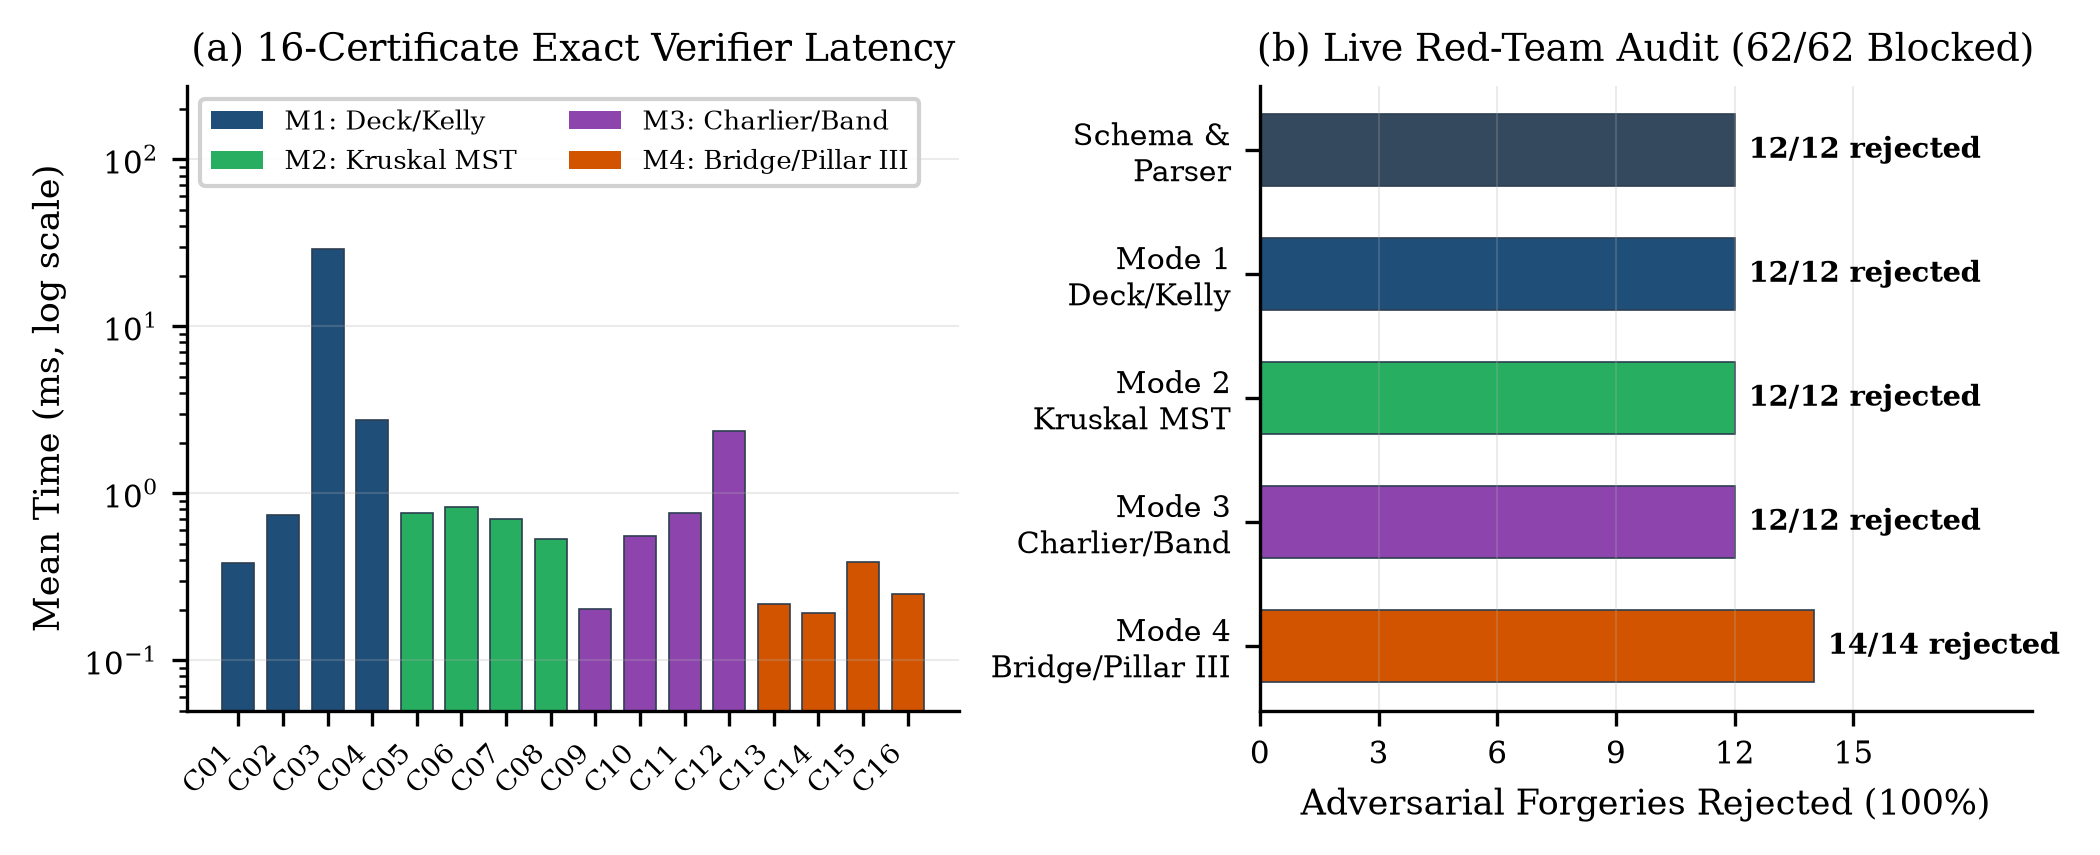
\includegraphics[width=\columnwidth]{figures/fig3_atlas_and_redteam.png}
\vspace{-1.3em}
\caption{\textbf{(a)}~Mean zero-float verification latency across all 16 canonical certificates ($0.192$--$28.989\,\mathrm{ms}$, log scale). \textbf{(b)}~Live adversarial red-team audit rejecting 62/62 forgeries across five attack classes with exact error-branch assertions.}
\label{fig:atlas}
\end{figure}

\paragraph{2. Hand-Verifiable Worked Exact Witnesses (One per Mode).}
To ensure complete standalone auditability directly from this manuscript:
\begin{itemize}[leftmargin=1.2em,itemsep=1pt,topsep=2pt]
  \item \textbf{Mode~1 (\texttt{C02}, $m{=}3$ Harary pair):} $G = K_3\sqcup K_1$ ($E_G=\{(0,1),(1,2),(0,2)\}$, degs $(0,2,2,2)$, $|\mathrm{Aut}|=6$) vs.\ $H = K_{1,3}$ ($E_H=\{(0,1),(0,2),(0,3)\}$, degs $(1,1,1,3)$, $|\mathrm{Aut}|=6$). Deleting any edge yields $K_{1,2}\sqcup K_1$, so $\mathcal{D}_E(G)=\mathcal{D}_E(H)$ while $\mathcal{D}(G)\ne\mathcal{D}(H)$; edge-Kelly gives $(3-1)\cdot s(K_2,G)=6=\sum_e 2$ and $(3-2)\cdot s(P_3,G)=3=\sum_e 1$.
  \item \textbf{Mode~2 (\texttt{C05}, $n{=}12, m{=}15$):} Triangle hubs $\{0,1,2\}$ (all deg~5), three twin $K_2$-pendants $\{(3,4),(5,6),(7,8)\}$ attached to hub~0, and three degree-2 twins $\{9,10,11\}$ adjacent to $\{1,2\}$. At $\Delta_0=3$ ($H_0=\{0,1,2\}$), Kruskal selects $\{9\}$ as the sole bridge ($1\le |H_0|-1=2$, core edges $3\le 4$), leaving 3 twin $K_2$-pendants on hub~0 ($3!$) and 2 non-bridge $\{1,2\}$-twins ($2!$), certifying $3!\cdot 2!=12 \mid 72 = |\mathrm{Aut}(G)|$, with 3 internal $\Phi_3$-zero-drop edges.
  \item \textbf{Mode~3 (\texttt{C11}, 4-var Vandermonde):} $P=\prod_{0\le i<j\le 3}(y_i-y_j)$ has $N_0=6$, 24 terms ($\pm 1$), $D_I(P)\equiv 0$, target $v=(3,2,1,0)$, $\|P\|_1/|c_v|=24$. Band $[t_0,t_1]=[1,2]$ gives $I_{\mathrm{lo}}=\{3\}$, $I_{\mathrm{mid}}=\{1,2\}$, $I_{\mathrm{hi}}=\{0\}$, $C_{\mathrm{const}}=\binom{3}{1}\binom{2}{1}\binom{1}{1}=6$, and $F_{\mathrm{mid}}(y_1,y_2)=y_1-y_2$ ($\|F_{\mathrm{mid}}\|_1=2\le 24$, $D_{I_{\mathrm{mid}}}(F_{\mathrm{mid}})\equiv 0$).
  \item \textbf{Mode~4 (\texttt{C13} \& \texttt{C14}):} In \texttt{C13}, $K_6$ hubs $\{0..5\}$ attach to $D=\{6,7,8,9\}\subset V_{<4}$ (root $v_0=6$, leaves $7\to\{0,1\}, 8\to\{2,3\}, 9\to\{4,5\}$); $Q_D\cong S_2\wr S_3$ has exact order $48=2^4\cdot 3$ (primes $\{2,3\}<4$, $48\le 64^6$). In \texttt{C14} ($\Delta=5$, $K_6$ hubs + 4 degree-2 twin classes $\{[11,12],[13,14],[15],[16,17]\}$), selecting 2/4 classes ($\ge 3/8$) gives $W_0=\{11,12,13,14\}$, preserves $2d_{K_0}(x)\ge d_G(x)$, and satisfies $\sum_{u\in H_5}(d_G(u)-d_{K_0}(u))=8=2\cdot|W_0|$.
\end{itemize}

\begin{table}[t]
\centering
\caption{Canonical 16-certificate \nolinkurl{EDGERECON-COGENTIC-CERT-1.0} atlas (\nolinkurl{results/exp1_certificate_atlas.json}; all 16 verified).}
\label{tab:atlas}
\scriptsize
\setlength{\tabcolsep}{2.1pt}
\resizebox{\columnwidth}{!}{%
\begin{tabular}{@{}l c l r@{}}
\toprule
Certificate ID & M & Exact Certified Witness Summary & ms \\
\midrule
\texttt{m1\_harary\_m2\_counterexample} & M1 & $2K_2$ vs.\ $K_{1,2}\sqcup K_1$: $\mathcal{D}_E{=}, \mathcal{D}{\ne}, |\mathrm{Aut}|{=}8,2$ & 0.384 \\
\texttt{m1\_harary\_m3\_counterexample} & M1 & $K_3\sqcup K_1$ vs.\ $K_{1,3}$: $\mathcal{D}_E{=}, \mathcal{D}{\ne}, |\mathrm{Aut}|{=}6,6$ & 0.743 \\
\texttt{m1\_muller\_dense\_n6\_iso\_kelly} & M1 & $n{=}6,m{=}11$: $2^{10}>6!$, 5 Kelly $\ZZ$-ids ok & 28.989 \\
\texttt{m1\_harary\_m5\_deck\_distinguished} & M1 & $C_5$ vs.\ lollipop ($m{=}5$): $\mathcal{D}_E\ne$, 4 Kelly ok & 2.730 \\
\texttt{m2\_kruskal\_n12\_hub\_twins\_exact\_aut} & M2 & $n{=}12,m{=}15$: $\prod\tilde{w}!{=}12\mid 72$, $\Phi_3$: 3 int. & 0.761 \\
\texttt{m2\_kruskal\_n14\_two\_tier\_dyadic} & M2 & $n{=}14,m{=}17$: 2 scales, $12\mid 96$, $\Phi_3$: 4 int. & 0.827 \\
\texttt{m2\_kruskal\_n24\_three\_tier\_dyadic} & M2 & $n{=}24,m{=}31$: 3 scales, $\prod\tilde{w}!{=}1728$, $\Phi_6$ ok & 0.697 \\
\texttt{m2\_kruskal\_n20\_dual\_cliques\_bridges} & M2 & $n{=}20,m{=}32$: 2 scales, $\prod\tilde{w}!{=}576$, $\Phi_3$ ok & 0.532 \\
\texttt{m3\_shift\_t1\_multilinear\_n2} & M3 & $M{=}4,N_0{=}2,t{=}1$: $\rho{=}4$, $|I_{1,1}|{=}11/12$ & 0.204 \\
\texttt{m3\_shift\_t1\_multilinear\_n4} & M3 & $M{=}8,N_0{=}4,t{=}1$: $\rho{=}16$, $|I_{3,3}|<69/80$ & 0.558 \\
\texttt{m3\_vandermonde4\_lemma43\_band} & M3 & $V_4$ ($N_0{=}6$): band $[1,2]\to$ deg-1, $\|F_{\mathrm{mid}}\|_1{=}2$ & 0.763 \\
\texttt{m3\_vandermonde5\_lemma43\_band} & M3 & $V_5$ ($N_0{=}10$): band $[1,3]\to$ deg-3, $\|F_{\mathrm{mid}}\|_1{=}6$ & 2.362 \\
\texttt{m4\_bridge\_d4\_wreath48\_vacuous2000} & M4 & $\Delta{=}4,R{=}6,|Q_D|{=}48$; $n_0{=}2000$ vacuous & 0.218 \\
\texttt{m4\_bridge\_d5\_pillar3\_r2\_active2001} & M4 & $\Delta{=}5,|Q_D|{=}6$; P3 $r{=}2$, exc.\ 8; $n_0{=}2001$ & 0.192 \\
\texttt{m4\_bridge\_d6\_pillar3\_r3\_active1e6} & M4 & $\Delta{=}6,|Q_D|{=}24$; P3 $r{=}3$, exc.\ 12; $n_0{=}10^6$ & 0.387 \\
\texttt{m4\_bridge\_d6\_beyond\_muller\_2pow1005} & M4 & $\Delta{=}6,|Q_D|{=}6$; $n_0{=}2^{1005}$ beats M\"uller! & 0.249 \\
\bottomrule
\end{tabular}}
\end{table}

\paragraph{3. 16-Certificate Atlas \& 66-Test Red-Team Audit (Table~\ref{tab:atlas}, Fig.~\ref{fig:atlas}).}
Table~\ref{tab:atlas} summarizes all 16 canonical certificates ($0.192$--$28.989\,\mathrm{ms}$). \texttt{tests/test\_\allowbreak suite.py} runs 66 pytest functions: 1 full replay of all 16 certificates, 3 raw-JSON parser guards (IEEE-754 float, \texttt{NaN}, duplicate keys), and 62 parametrized live adversarial forgeries (12 schema/parser + 12 each for Modes~1--3 + 14 for Mode~4, covering self-loops, non-monotone Kruskal orderings, forged MST edges, non-shift-invariant polynomials, non-uniform Lemma~4.3 partitions, disconnected bridge subsets, broken open-twin classes, $r\ge\Delta_{k-1}$ leaf-stratum violations, split size-4 twin classes, $<3/8$ sampling ratios, and half-degree violations), each asserting an exact regex match on its intended \texttt{CertificateError} branch. \texttt{scripts/verify\_\allowbreak all.py} enforces all 5 gates including strict axiom whitelisting and a 40-file SHA-256 manifest.

\section{Conclusion}\label{sec:conc}
We built an independent, explicitly scoped, zero-floating-point verification stack for Google Research Cogentic's unconditional linear-density edge reconstruction theorem ($m\ge 1000\,n_0$)~\cite{cogentic2026edgerecon}, uniting 18 constructive Lean~4.35.0 theorems (zero \texttt{sorry}, zero \texttt{Classical.choice}), the pure-\texttt{int}/\texttt{Fraction} 4-mode auditor \texttt{EDGERECON-COGENTIC-CERT-1.0}, 16 canonical exact witnesses spanning Harary's $m\le 3$ boundary to $n_0=2^{1005}$ beyond M\"uller, and 62/62 live adversarial forgery rejections.

{\footnotesize
\bibliographystyle{plain}
\bibliography{references}}
\end{document}
